\documentclass[twoside, 10pt]{article}

\usepackage{geometry}
\geometry{outer=2em, inner=2.2cm, top=6em, bottom=4em, headheight=\paperheight}
\usepackage[export]{adjustbox}
\usepackage{array}
\usepackage{amsmath}
\usepackage{amsfonts}
\usepackage{fancyhdr}
\pagestyle{fancy}
\fancyhf{}
\lhead{Algebra II - BASE}
\chead{Function  Characteristics - End behaviors}
\rhead{Action Opportunity A, Page \thepage}
\usepackage{lastpage}
\usepackage{xcolor}
\usepackage{enumitem}
\usepackage{pifont}
\usepackage{graphicx}
\graphicspath{{../img}}
\usepackage{pgfplots}
\pgfplotsset{compat=1.18}
\usepackage{tabularx}
\usepackage{tikz}
\usetikzlibrary{patterns}

\newcommand{\R}{\mathbb R}
\newcommand{\e}{{\rm e}}
\newcommand{\pobr}[1]{\left\langle#1\right\rangle}
\newcommand{\norm}[1]{\lVert #1 \rVert}
\newcommand{\abs}[1]{\lvert #1 \rvert}

\DeclareMathOperator{\xd}{d\!}
\DeclareMathOperator{\proj}{proj}

\title{}
\date{}

\begin{document}
\noindent
{\large
First Name \rule{6em}{.1pt}\hspace{\stretch{1}}Last Name \rule{6em}{.1pt}\hspace{\stretch{1}} Date \rule{1.5em}{.1pt} -- \rule{1.5em}{.1pt} -- \rule{1.5em}{.1pt}\hspace{\stretch{1}} Period \rule{2em}{.1pt}\hspace{\stretch{1}} Score \rule{2em}{.1pt}
}
\vspace{1em}

\begingroup
\renewcommand{\arraystretch}{1.5}
\begin{center}
\tiny
{
\begin{tabularx}{\textwidth}{|X|X|X|X|X|X|}
\hline
\bf BE PRECISE & \centerline{Integrating} & \centerline{Applying} & \centerline{Practicing} & \centerline{Acquiring} & \centerline{Awaiting Evidence} \\
\hline
I can calculate accurately and efficiently, and be precise in all of my math.&
Selects and applies the correct procedure and solves all routine AND integrating problems.

AND

Expresses the answer to the correct level of precision needed for the problem (including the correct rounding, units, math symbols, labeling, graphing, vocab…)
&Selects and applies the correct procedure and solves all routine problems.


AND

Expresses the answer to the correct level of precision needed for the problem (including the correct rounding, units, math symbols, labeling, graphing, vocab…)
&Selects and applies the correct procedure and solves most routine problems.


AND

Expresses the answer to the correct level of precision needed for the problem (including the correct rounding, units, math symbols, labeling, graphing, vocab…)
&Selects and applies the correct procedure and solves some routine problems.


AND

Attempts to express the answer to the correct level of precision needed for the problem (including the correct rounding, units, math symbols, labeling, graphing, vocab…).
&Selects and attempts to apply the correct procedure for some routine problems.\\
\hline
\bf Criteria&\multicolumn{5}{l|}{\parbox[c][4em]{.8\textwidth}{}}\\
\hline
\end{tabularx}
}
\end{center}
\endgroup
\vspace{1em}

{\noindent\bf Problem.}

\begin{enumerate}[leftmargin=*]
\item  Shade the segment represented by the interval \([-7, 0)\) on the number line. Use $\bullet$ to indicate a closed endpoint, and $\circ$ to indicate an open endpoint.
\begin{center}
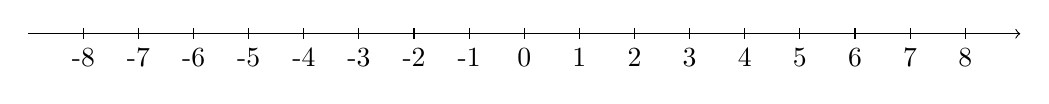
\begin{tikzpicture}[scale=0.7]
  \draw[->] (-9,0) -- (9,0);
  \foreach \x in {-8,..., 8}
    \draw (\x,0.1) -- (\x,-0.1) node[below] {\x};
\end{tikzpicture}
\end{center}
\item  Shade the segment represented by the interval \((-3, \infty)\) on the number line. Use $\bullet$ to indicate a closed endpoint, and $\circ$ to indicate an open endpoint.
\begin{center}
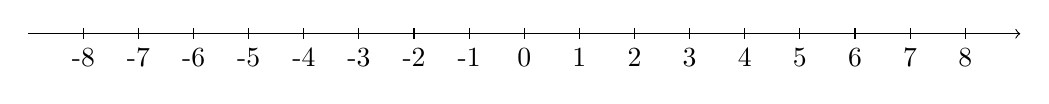
\begin{tikzpicture}[scale=0.7]
  \draw[->] (-9,0) -- (9,0);
  \foreach \x in {-8,..., 8}
    \draw (\x,0.1) -- (\x,-0.1) node[below] {\x};
\end{tikzpicture}
\end{center}
\item The interval represented by the shaded segment below is \rule{10em}{0.1pt} .
\begin{center}
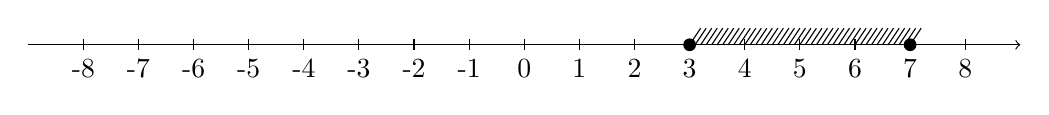
\begin{tikzpicture}[scale=0.7]
  \draw[->] (-9,0) -- (9,0);
  \foreach \x in {-8,..., 8}
    \draw (\x,0.1) -- (\x,-0.1) node[below] {\x};
  \foreach \x in {3,3.1, ..., 7.1}
    \draw (\x, 0) -- (\x+0.2, 0.3);
\draw[fill=black] (3,0) circle(3pt);
\draw[fill=black] (7,0) circle(3pt);
\end{tikzpicture}
\end{center}
\item
The following graph shows the state of an object cooling over time:

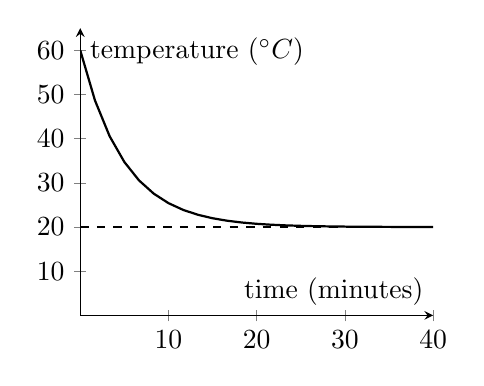
\begin{tikzpicture}
\begin{axis}[
axis lines=middle,
xlabel={time (minutes)},
ylabel={temperature (${}^\circ C$)},
ymin=0, ymax = 65,
domain=0:40,
ytick distance=10,
grid style={draw=gray!80, dashed},
width=0.5\textwidth,
]
\addplot[thick]{20 + 40*e^(-0.2*x) };
\addplot[dashed]{20};
\end{axis}
\end{tikzpicture}
\begin{enumerate}
\item 
What is the temperature of the object as time approaches infinity? \rule{4em}{0.1pt}.
\vspace{\stretch{1}}
\item
What can you infer about the room temperature in which this cooling process was taking place? \rule{4em}{0.1pt}.
\vspace{\stretch{1}}
\end{enumerate}
\clearpage
\noindent{\bf Direction.} Describe the end behaviors of the graphs below. If the graph doesn't have a definite end behavior, put ``N/A''.
\item
\begin{center}
\begin{tabular}{cc}
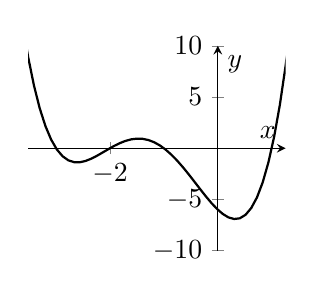
\begin{tikzpicture}[baseline={(current bounding box.center)}]
\begin{axis}[
xlabel={$x$},
ylabel={$y$},
axis lines=middle,
ymin=-10, ymax=10,
domain=-5:5.5,
samples=100,
width=0.4\textwidth,
grid style={draw=gray!80, dashed}
]
\addplot[thick]{(x-1)*(x+1)*(x+2)*(x+3)};
\end{axis}
\end{tikzpicture}
&\parbox{0.45\textwidth}{
$y=x^4 + 5 x^3 + 5 x^2 - 5 x - 6$.\\[1em]
As $x$ approaches $\infty$, $y$ approaches \rule{8em}{.1pt}.\\[1em]
As $x$ approaches $-\infty$, $y$ approaches \rule{8em}{.1pt}.\\[1em]
Does the graph have an absolute maximum?  \rule{4em}{.1pt}.\\[1em]
Does the graph have an absolute minimum?  \rule{4em}{.1pt}.}
\end{tabular}
\end{center}
\vspace{\stretch{1}}
\item
\begin{center}
\begin{tabular}{cc}
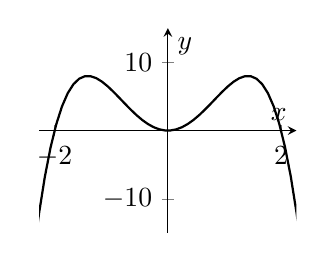
\begin{tikzpicture}[baseline={(current bounding box.center)}]
\begin{axis}[
xlabel={$x$},
ylabel={$y$},
axis lines=middle,
ymin=-15, ymax=15,
domain=-5:5,
samples=100,
width=0.4\textwidth,
grid style={draw=gray!80, dashed}
]
\addplot[thick]{-2*x^4+8*x^2)};
\end{axis}
\end{tikzpicture}
&\parbox{0.45\textwidth}{
$y=-2x^4 + 8x^2$.\\[1em]
As $x$ approaches $\infty$, $y$ approaches \rule{8em}{.1pt}.\\[1em]
As $x$ approaches $-\infty$, $y$ approaches \rule{8em}{.1pt}.\\[1em]
Does the graph have an absolute maximum?  \rule{4em}{.1pt}.\\[1em]
Does the graph have an absolute minimum?  \rule{4em}{.1pt}.}
\end{tabular}
\end{center}
\vspace{\stretch{1}}
\item
\begin{center}
\begin{tabular}{cc}
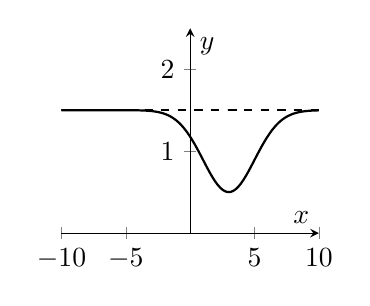
\begin{tikzpicture}[baseline={(current bounding box.center)}]
\begin{axis}[
xlabel={$x$},
ylabel={$y$},
axis lines=middle,
domain=-10:10,
ymax=2.5, ymin=0,
samples=100,
width=0.4\textwidth,
grid style={draw=gray!80, dashed}
]
\addplot[thick]{-e^(-(x-3)^2/8)+1.5};
\addplot[thick,dashed]{1.5};
\end{axis}
\end{tikzpicture}
&\parbox{0.45\textwidth}{
$\displaystyle y=-e^{-(x-3)^2/8}+1.5$.\\[1em]
As $x$ approaches $\infty$, $y$ approaches \rule{8em}{.1pt}.\\[1em]
As $x$ approaches $-\infty$, $y$ approaches \rule{8em}{.1pt}.\\[1em]
Does the graph have an absolute maximum?  \rule{4em}{.1pt}.\\[1em]
Does the graph have an absolute minimum?  \rule{4em}{.1pt}.}
\end{tabular}
\end{center}
\vspace{\stretch{1}}
\item
\begin{center}
\begin{tabular}{cc}
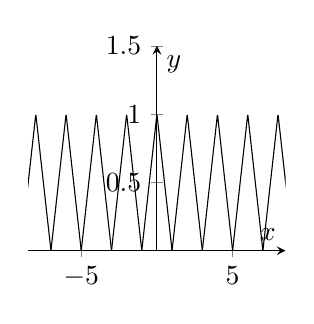
\begin{tikzpicture}[baseline={(current bounding box.center)}]
\begin{axis}[
xlabel={$x$},
ylabel={$y$},
axis lines=middle,
ymin=0, ymax=1.5,
xmin=-8.5, xmax=8.5,
samples=100,
width=0.4\textwidth,
grid style={draw=gray!80, dashed}
]
\foreach \k in {-5, ..., 5}
  \addplot[domain=-1+2*\k: 1+2*\k]{-abs(x-2*\k)+1};
\end{axis}
\end{tikzpicture}
&\parbox{0.45\textwidth}{
$y=f(x)$ is a periodic function that repeats the same pattern over and over.\\[1em]
As $x$ approaches $\infty$, $y$ approaches \rule{8em}{.1pt}.\\[1em]
As $x$ approaches $-\infty$, $y$ approaches \rule{8em}{.1pt}.\\[1em]
Does the graph have an absolute maximum?  \rule{4em}{.1pt}.\\[1em]
Does the graph have an absolute minimum?  \rule{4em}{.1pt}.}
\end{tabular}
\end{center}
\vspace{\stretch{1}}
\end{enumerate}
\end{document}